% Wallets workstream: results. Every number traces to data/research/flb_wallets/ (file named per paragraph).
This subsection answers the four questions of the wallets workstream in turn: how Polymarket prices
longshots, which wallets buy them, how concentrated and persistent wallet profits are, and how
retail inflows and cross-venue prices behave.

\subsubsection{Polymarket calibration and the bias by group}\label{sec:res-wallets-calib}

% source: data/research/flb_wallets/calib_slopes.csv, calib_market.csv
\Cref{tab:wallets-calib} and \cref{fig:wallets-calib} summarise calibration on Polymarket. Measured 24 hours before the
information time, the pooled calibration slope is $\hat\beta=0.99$ (SE 0.15; 2{,}121
markets), so $\beta=1$ is not rejected ($t=-0.1$). The slope is 0.91 (SE 0.14) one hour
before and 0.84 (SE 0.17) a week before. Weighting every sampled market equally gives
0.97 (SE 0.05). The slope is 1.28 in H1 and 0.97 in H2. By group, the 24-hour
slopes are Sports 1.00, Politics 1.15, Weather 0.71, Entertainment 1.20, Mentions 0.84, Science \& Tech 0.99, Other 0.82; 7 of the 7 are within two standard errors of one (\cref{tab:wallets-calib}).

Returns by price bucket are noisier. Buying every side priced at most 10\cents{} 24 hours
ahead returns 84.5\% ($t=0.5$) per dollar market-weighted, $-$16.5\% ($t=-0.2$) volume-weighted and 64.9\% ($t=0.8$) with equal weights. Buying
every side priced at least 90\cents{} returns 1.9\% ($t=2.5$) and 2.3\% ($t=4.8$). Longshot returns are imprecise because a
handful of 1--2\cents{} winners carry large design weights. The calibration slope pools all price levels and is the
more reliable summary.

% source: data/research/flb_wallets/trade_flb.csv (ret_n, dollar-weighted)
At the level of fills the bias is clear. Buying a longshot before the information time and holding it to
settlement returns $-$53.8\% ($t=-2.8$) per dollar net of fees; buying a favourite returns 2.2\% ($t=3.5$). The signs are the
same in every group: longshot buys lose between 48\% and 71\% per dollar (significant at
5\% in 5 of the 7 groups), and favourite buys earn between 1.1\% and 3.5\%
(significant in 4; \cref{tab:wallets-calib}). The longshot loss is larger for takers ($-$71.2\% ($t=-5.9$)) than for
makers ($-$33.3\% ($t=-1.2$)), and larger in H1 ($-$90.9\% ($t=-18.7$)) than in H2 ($-$30.2\% ($t=-1.0$)). Favourites earn 3.9\% ($t=6.9$) in H1 and
1.4\% ($t=1.7$) in H2. The two measures weight markets and moments differently. The fill-level return weights each
dollar actually spent, including purchases in the last hours before the information time. The market-level
calibration takes one price per market a day ahead, where the bias is weak. \Cref{sec:res-xs} reports
the corresponding Kalshi estimates.

\begin{figure}[t]
\centering
% source: data/research/flb_wallets/calib_market.csv, trade_flb.csv
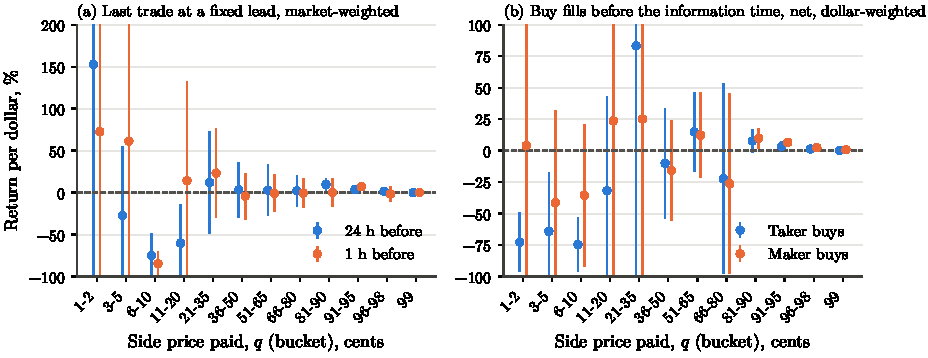
\includegraphics[width=\textwidth]{figures/fig_wallets_calib.pdf}
\caption{Return per dollar by side-price bucket on Polymarket. (a) Last trade 24 hours and 1 hour before the information time, both sides of each market, market-weighted with design weights, gross. (b) Buy fills before the information time held to settlement, net of taker fees, dollar-weighted, by liquidity role. Bars are 95\% confidence intervals clustered by event, truncated at the axis limits.}\label{fig:wallets-calib}
\end{figure}

\begin{table}[t]
\centering
\small
\begin{threeparttable}
\caption{Polymarket calibration and longshot returns by group}\label{tab:wallets-calib}
\footnotesize
\setlength{\tabcolsep}{4pt}
% source: data/research/flb_wallets/calib_slopes.csv, calib_market.csv (lead_h=24, market-weighted), trade_flb.csv (ret_n, dollar)
\begin{tabular}{lrcccccc}
\toprule
& & \multicolumn{4}{c}{Last trade 24\,h before $t^{\mathrm{info}}$} & \multicolumn{2}{c}{Buy fills before $t^{\mathrm{info}}$} \\
\cmidrule(lr){3-6}\cmidrule(lr){7-8}
& & $\hat\beta$ (SE) & $\hat\beta$ (SE) & $\ret$, \LS & $\ret$, \FAV & $\ret$, \LS & $\ret$, \FAV \\
& Markets & design & sample & \% ($t$) & \% ($t$) & \% ($t$) & \% ($t$) \\
\midrule
All markets & 2{,}121 & 0.99 (0.15) & 0.97 (0.05) & 84.5 (0.5) & 1.9 (2.5) & $-$53.8 ($-$2.8) & 2.2 (3.5) \\
\addlinespace
Sports & 285 & 1.00 (0.24) & 1.08 (0.18) & $-$93.6 ($-$20.3) & 5.7 (3.6) & $-$60.1 ($-$2.2) & 3.3 (2.0) \\
Politics & 416 & 1.15 (0.18) & 1.05 (0.13) & $-$80.3 ($-$8.3) & 0.4 (0.5) & $-$48.0 ($-$1.5) & 2.1 (2.0) \\
Weather & 303 & 0.71 (0.25) & 0.74 (0.14) & 257.7 (0.7) & 0.4 (0.5) & $-$70.6 ($-$6.2) & 1.4 (7.1) \\
Entertainment & 406 & 1.20 (0.19) & 1.24 (0.15) & $-$84.4 ($-$8.3) & 1.2 (2.4) & $-$59.2 ($-$3.9) & 2.0 (3.2) \\
Mentions & 227 & 0.84 (0.14) & 0.77 (0.13) & $-$88.3 ($-$7.3) & 6.7 (7.7) & $-$57.4 ($-$2.8) & 3.5 (1.6) \\
Science \& Tech & 289 & 0.99 (0.16) & 1.04 (0.13) & $-$26.1 ($-$0.5) & $-$1.2 ($-$0.7) & $-$61.0 ($-$2.8) & 1.1 (1.8) \\
Other & 195 & 0.82 (0.15) & 0.89 (0.13) & 18.3 (0.3) & $-$3.4 ($-$1.4) & $-$49.1 ($-$1.6) & 1.4 (1.4) \\
\addlinespace
H1 & 912 & 1.28 (0.16) & 1.06 (0.09) & $-$36.1 ($-$1.5) & 0.2 (0.2) & $-$90.9 ($-$18.7) & 3.9 (6.9) \\
H2 & 1{,}209 & 0.97 (0.16) & 0.91 (0.06) & 93.3 (0.5) & 2.0 (2.5) & $-$30.2 ($-$1.0) & 1.4 (1.7) \\
\bottomrule
\end{tabular}
\begin{tablenotes}\footnotesize
\item Sample: stratified random sample of resolved in-scope Polymarket markets (\$1k--\$6M), January 2024
  to October 2026. Left block: one observation per side of each market with a trade at least 24\,h before
  its information time $t^{\mathrm{info}}$; $\beta$ from \eqref{eq:logit} on the outcome-0 side, with design
  weights or with every sampled market weighted equally (``sample''); \LS: $\q\le10\cents$, \FAV: $\q\ge90\cents$; returns
  $\ret$ in \% per dollar, gross (Polymarket charged no fees before 2026), market-weighted (design weights).
  H1: markets resolving January 2024 to May 2025; H2: June 2025 to October 2026.
  Right block: buy fills (maker and taker) before $t^{\mathrm{info}}$, held to settlement, \% per dollar
  net of taker fees, dollar-weighted (notional $\times$ design weight). $t$-statistics in parentheses;
  standard errors clustered by event.
\end{tablenotes}
\end{threeparttable}
\end{table}

\subsubsection{Who buys longshots}\label{sec:res-wallets-who}

% source: data/research/flb_wallets/who_share.csv (dim=cls), ls_flow.csv, class_pnl.csv
\Cref{tab:wallets-class} describes the five classes. Occasional small wallets (``retail'') make
31.3\% of buy fills and 12.4\% of dollars bought, across 175{,}734 wallets.
Market-maker-like wallets make 33.3\% of fills, and whales 21.9\% of dollars from only
1{,}677 wallets.

Longshots are a large share of what small wallets and market makers \emph{buy}, but a small share of what
any class \emph{spends}:
\begin{itemize}
  \item Longshots are 11.5\% of retail buy fills, 15.7\% of active-retail fills and 21.8\% of
    market-maker fills, but only 1.5\% of mid-size and 0.2\% of whale fills
    (\cref{fig:wallets-lsshare}).
  \item Because longshots are cheap, they are at most 1.3\% of any
    class's dollars bought.
  \item Favourites take between 5.7\% and
    14.8\% of each class's dollars: most for
    active retail and retail, least for whales.
\end{itemize}

Net flows show who takes the other side. Counting every buy and sell before the information time,
retail wallets are the clear net buyers of longshots: 0.43\% of the dollars they trade
($t=3.9$), as takers (0.47\%, $t=2.7$) and with resting orders (0.39\%,
$t=2.4$). Net flows sum to zero across classes, and retail makes 86\% of all net longshot
buying. The other classes are close to flat on net: active retail 0.04\% ($t=0.4$), mid-size wallets $-$0.06\% ($t=-1.0$), whales $-$0.06\% ($t=-1.6$), market makers $-$0.16\% ($t=-1.3$). None of these is individually significant
($|t|\leq1.6$). The longshot buying of small, occasional wallets is thus absorbed by many counterparties,
not by one class of professional sellers. That small accounts tilt towards lottery-like payoffs matches the evidence on
individual investors in equity markets \citep{kumar2009}.

The returns on these purchases differ by class (\cref{fig:wallets-classret}). Per dollar, net longshot returns
are $-$36.3\% ($t=-1.4$) for retail, $-$59.4\% ($t=-3.0$) for active retail and $-$42.3\% ($t=-1.6$) for market makers;
the few longshots bought by mid-size wallets and whales lose 90\% and 100\% of
their cost. Across all
price levels, class PnL per dollar traded is $-$2.1\% ($t=-0.8$) for retail, 14.1\% ($t=2.5$) for
active retail, $-$6.3\% ($t=-1.2$) for mid-size wallets, 5.3\% ($t=1.1$) for whales and $-$10.8\% ($t=-1.4$) for market
makers (\cref{tab:wallets-class}). Only the figure for active retail is significant at the 5\% level.
\Cref{tab:wallets-robust} in \cref{app:wallets} shows that the ordering of longshot shares survives every change of cut-off.

% source: data/research/flb_wallets/who_share.csv (dims size_bucket, lb)
Fill size gives the same gradient without any classification (\cref{tab:wallets-sizeage}). Longshots are
23.1\% of buy fills of at most \$10, 2.4\% of \$10--100 fills,
0.7\% of \$100--1k fills and 0.2\% of fills above \$1{,}000. Per dollar,
however, the small longshot purchases lose least: $-$22.2\% ($t=-0.6$) for fills of at most \$10,
against $-$48.4\% ($t=-2.4$) at \$10--100 and $-$77.6\% ($t=-4.5$) at
\$100--1k. All-time
leaderboard wallets put 6.8\% of their buy fills into longshots, against 15.4\% for other
wallets.

% source: data/research/flb_wallets/hold_exit.csv
Do longshot buyers hold to settlement? \Cref{tab:wallets-holdexit} in \cref{app:wallets} follows each position
opened by a buy. Retail sells at least half of 41.7\% of its longshot positions before the close, active
retail 6.9\% and market makers 54.7\%. For longshot entries, the realised PnL exceeds
the hold-to-settlement PnL by 23.2\% ($t=2.2$) of cost: the shares sold were worth less at settlement than their sale
price, as expected if longshots are overpriced when they are sold. Across all positions the difference is
$-$1.4\% ($t=-1.3$), and for favourite entries $-$1.2\% ($t=-2.1$). Selling favourites early forgoes some of their small
positive return.

\begin{figure}[t]
\centering
% source: data/research/flb_wallets/who_share.csv
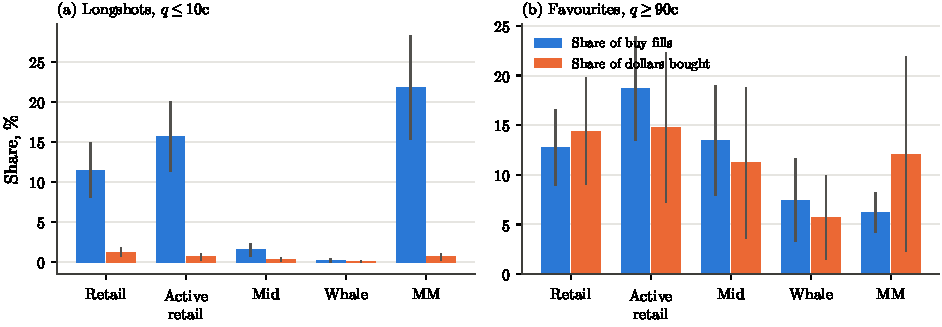
\includegraphics[width=\textwidth]{figures/fig_wallets_lsshare.pdf}
\caption{Longshot ($q\le10$c) and favourite ($q\ge90$c) shares of buying by wallet class: share of design-weighted buy fills and of dollars bought, buy fills before the information time. Bars are 95\% confidence intervals clustered by event.}\label{fig:wallets-lsshare}
\end{figure}

\begin{figure}[t]
\centering
% source: data/research/flb_wallets/who_class_cbucket.csv
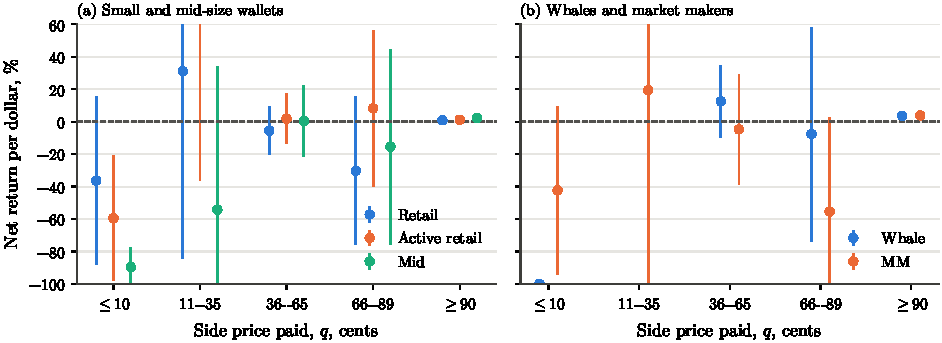
\includegraphics[width=\textwidth]{figures/fig_wallets_classret.pdf}
\caption{Net return per dollar of buy fills by wallet class and side price, held to settlement, dollar-weighted, buy fills before the information time. Bars are 95\% confidence intervals clustered by event.}\label{fig:wallets-classret}
\end{figure}

\begin{table}[t]
\centering
\small
\begin{threeparttable}
\caption{Who buys longshots: buying, returns and PnL by wallet class}\label{tab:wallets-class}
% source: data/research/flb_wallets/who_share.csv (dim=cls, half=All), ls_flow.csv (half=All, role=all), class_pnl.csv (half=All)
\footnotesize
\setlength{\tabcolsep}{4pt}
\begin{tabular}{lrrrrrrccc}
\toprule
& & \multicolumn{2}{c}{Share of buying} & \multicolumn{2}{c}{\LS{} share} & \FAV{} share & \LS{} $\ret$ & Net \LS{} flow & PnL per \$ \\
\cmidrule(lr){3-4}\cmidrule(lr){5-6}\cmidrule(lr){7-7}\cmidrule(lr){8-8}\cmidrule(lr){9-9}\cmidrule(lr){10-10}
Class & Wallets & fills & \$ & fills & \$ & \$ & \% ($t$) & \% ($t$) & \% ($t$) \\
\midrule
Retail & 175{,}734 & 31.3 & 12.4 & 11.5 & 1.3 & 14.4 & $-$36.3 ($-$1.4) & 0.43 (3.9) & $-$2.1 ($-$0.8) \\
Active retail & 6{,}431 & 31.9 & 24.1 & 15.7 & 0.7 & 14.8 & $-$59.4 ($-$3.0) & 0.04 (0.4) & 14.1 (2.5) \\
Mid & 15{,}393 & 3.2 & 20.5 & 1.5 & 0.3 & 11.2 & $-$89.6 ($-$14.9) & $-$0.06 ($-$1.0) & $-$6.3 ($-$1.2) \\
Whale & 1{,}677 & 0.2 & 21.9 & 0.2 & 0.1 & 5.7 & $-$100.0 ($<-$100) & $-$0.06 ($-$1.6) & 5.3 (1.1) \\
MM & 3{,}589 & 33.3 & 21.1 & 21.8 & 0.7 & 12.1 & $-$42.3 ($-$1.6) & $-$0.16 ($-$1.3) & $-$10.8 ($-$1.4) \\
\bottomrule
\end{tabular}
\begin{tablenotes}\footnotesize
\item Classes are assigned to each fill from the wallet's history before it (\cref{sec:method-wallets}).
  Wallets: distinct wallets with at least one buy in the class (a wallet can change class over time).
  Shares of buying and longshot ($\q\le10\cents$) / favourite ($\q\ge90\cents$) shares use buy fills before
  $t^{\mathrm{info}}$, in \% of design-weighted fills or dollars. Longshot $\ret$: net return per dollar of
  those longshot buys held to settlement, dollar-weighted. Net LS flow: net longshot dollars bought per
  dollar traded (buys and sells, both roles; positive = net buyer of longshots). PnL per \$: exact
  wallet-market PnL \eqref{eq:wallets-pnl} net of fees per dollar traded, class at the wallet's first fill
  in the market. $t$-statistics clustered by event.
\end{tablenotes}
\end{threeparttable}
\end{table}

\subsubsection{Profit concentration and persistence}\label{sec:res-wallets-skill}

% source: data/research/flb_wallets/summary.json:concentration
The accounting identity holds in the data. In 99.95\% of the
2{,}197 fee-free markets the PnL of all wallets sums to zero within $10^{-6}$ of turnover, and the
YES-equivalent positions sum to zero in 97.8\%. In fee markets the residual is
the fee charged in shares. PnL is therefore a transfer between wallets. Of 237{,}569
wallets, 50.7\% end with positive PnL in the sampled markets. The gains are highly
concentrated (\cref{tab:wallets-skill}, \cref{fig:wallets-lorenz}):
\begin{itemize}
  \item the top 1\% of wallets take 85\% of all gains and the top 0.1\%
    take 51\%;
  \item 220 wallets hold half of all gains;
  \item the Gini coefficient of gains among winners is 0.97.
\end{itemize}
Losses are less concentrated (Gini 0.95; 326 wallets
for half of all losses), and dollar volume is concentrated to a similar degree (Gini 0.96).
The 96 all-time leaderboard wallets in the sample take 11.8\% of gains on
10.4\% of volume. \citet{akey2026} report a similar concentration of profits across all
Polymarket users, and equity markets show the same pattern of losses spread over many individual traders
\citep{barberodean2000,barberleeliuodean2009}.

% source: data/research/flb_wallets/summary.json:persistence, persistence.csv
Concentration alone does not show skill: a market that pays out at long odds produces a few very large winners
by chance. We therefore rank the 719 wallets active in both halves on their shrunk H1
return \eqref{eq:wallets-shrink} and follow their H2 return (\cref{fig:wallets-persist}):
\begin{itemize}
  \item the rank correlation is 0.02 (95\% CI $-$0.06 to
    0.10), and 0.02 without shrinkage;
  \item the top H1 quintile earns $-$7.8\% per dollar relative to the bottom quintile in H2
    ($t=-1.2$);
  \item edge versus entry price, which removes favourite-versus-longshot style, has a rank correlation of
    $-$0.03.
\end{itemize}
The luck placebo gives a benchmark. With outcomes redrawn from the last pre-information price, the same wallets
and trades would produce a mean rank correlation of 0.15 (5th--95th percentile
0.09 to 0.20). That persistence comes from trading at prices
better or worse than the last trade before the information time. The actual correlation on the placebo sample,
$-$0.01, lies below all 200 placebo draws. So the
price advantage measured against the last trade does not persist in realised returns. That is consistent with
the last trade containing bid--ask bounce and with resting orders being filled when prices move against them.
Likewise, 5.1\% of wallets with at least 20 markets have a PnL $t$-statistic above 2,
against 7.0\% under the placebo. In this sample we find no persistent skill in
wallet returns, whether measured by raw returns, shrunk returns or edge versus entry price. This contrasts
with the persistence that \citet{barberleeliuodean2014} document among Taiwanese day traders. It also contrasts
with the persistent skilled minority that \citet{gomezcram2026} report from Polymarket's full trade record, and
agrees with the modest, possibly selection-driven persistence in \citet{akey2026}. Our panel is shorter and
covers only the sampled markets of each wallet, so it has less power to detect skill. Within it, the
concentration of gains is consistent with what a market with long-odds payoffs produces by chance.

\begin{figure}[t]
\centering
% source: data/research/flb_wallets/lorenz.csv
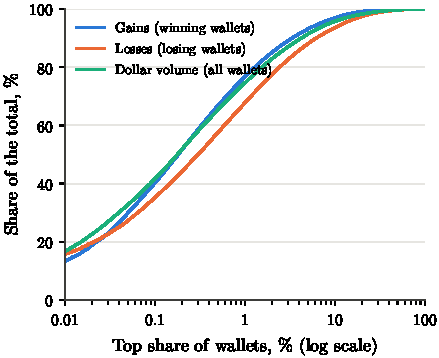
\includegraphics[width=0.55\textwidth]{figures/fig_wallets_lorenz.pdf}
\caption{Concentration of wallet outcomes: share of all gains (winning wallets), all losses (losing wallets) and all dollar volume held by the top $x$\% of wallets (equal shares would give $x$\%). Exact trade-based PnL over the sampled markets, net of fees.}\label{fig:wallets-lorenz}
\end{figure}

\begin{figure}[t]
\centering
% source: data/research/flb_wallets/persistence.csv, summary.json:persistence
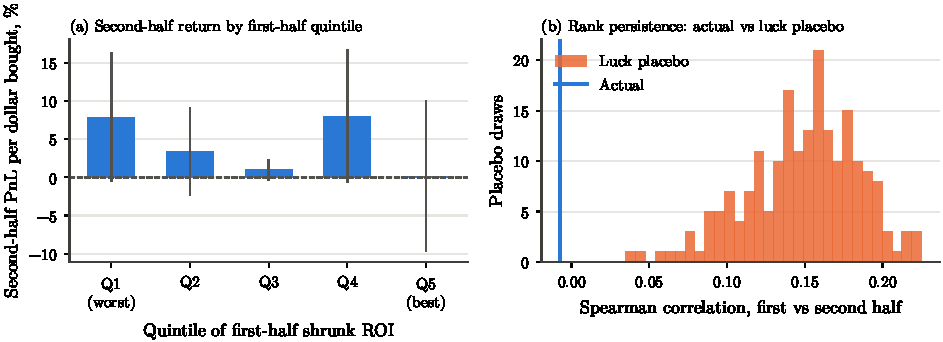
\includegraphics[width=\textwidth]{figures/fig_wallets_persist.pdf}
\caption{Persistence of wallet returns. (a) H2 PnL per dollar bought by quintile of shrunk H1 return, wallets active in both halves, with 95\% bootstrap intervals. (b) Rank correlation between halves under 200 draws of the luck placebo (outcomes redrawn from the last pre-information price) and the actual value on the same wallets.}\label{fig:wallets-persist}
\end{figure}

\begin{table}[t]
\centering
\small
\begin{threeparttable}
\caption{Profit concentration and persistence of wallet performance}\label{tab:wallets-skill}
% source: data/research/flb_wallets/summary.json:concentration, summary.json:persistence
\begin{tabular}{lr}
\toprule
\multicolumn{2}{l}{\emph{Concentration of PnL across wallets}} \\
Wallets in the sample & 237{,}569 \\
Share with positive PnL (\%) & 50.7 \\
Share of all gains: top 0.1\% / 1\% / 10\% of wallets (\%) & 51 / 85 / 99 \\
Wallets holding half of all gains / half of all losses & 220 / 326 \\
Gini: gains (winners) / losses (losers) / dollar volume & 0.97 / 0.95 / 0.96 \\
Leaderboard wallets: number / share of gains / share of volume (\%) & 96 / 11.8 / 10.4 \\
\addlinespace\multicolumn{2}{l}{\emph{Persistence, H1 $\to$ H2}} \\
Wallets active in both halves & 719 \\
Spearman, raw H1 ROI vs H2 ROI [95\% CI] & 0.02 [$-$0.06, 0.10] \\
Spearman, shrunk H1 ROI vs H2 ROI [95\% CI] & 0.02 [$-$0.06, 0.10] \\
Spearman, edge vs entry price, H1 vs H2 & $-$0.03 (694 wallets) \\
H2 ROI, top minus bottom quintile (\%, $t$) & $-$7.8 ($-$1.2) \\
Luck placebo: Spearman mean [5th, 95th pct.] & 0.15 [0.09, 0.20] \\
Actual Spearman on the placebo sample (percentile) & $-$0.01 (0) \\
Wallets with $\geq$20 markets: share with $t>2$, actual / placebo (\%) & 5.1 / 7.0 \\
\bottomrule
\end{tabular}
\begin{tablenotes}\footnotesize
\item PnL is exact trade-based PnL \eqref{eq:wallets-pnl} summed over the sampled markets, net of taker fees.
  Leaderboard: wallets on Polymarket's all-time overall, politics or sports top-100 (measured after the
  fact). Persistence: wallets with $\geq5$ markets and $\geq\$50$ bought in each half; shrunk ROI
  \eqref{eq:wallets-shrink}; edge = buy return minus its price bucket's mean in that half. The placebo redraws
  outcomes from the last pre-information price (200 draws). CIs from 500 wallet bootstraps.
\end{tablenotes}
\end{threeparttable}
\end{table}

\subsubsection{Retail inflows, attention and herding}\label{sec:res-wallets-dyn}

% source: data/research/flb_wallets/summary.json:dynamics, inflow_weekly.csv, inflow_events.csv, newwallet_monthly.csv, who_share.csv (dim=age_bucket)
Account creation dates are available for 5{,}144 wallets of the address-selected subset.
\Cref{fig:wallets-inflow}(a) plots their creation dates by week. The ratio of creations in the 14 days around each
event to the rate four to eight weeks before, with 95\% intervals, is: US election 2024 2.01 [1.64, 2.47]; Super Bowl LIX 0.40 [0.32, 0.49]; Papal conclave 2025 1.03 [0.76, 1.40]; NYC mayor 2025 2.59 [1.99, 3.37]; Super Bowl LX 1.26 [0.96, 1.65]. Each event window contains between 64 and
180 creations. Creations rise significantly around US election 2024 and NYC mayor 2025. They fall around Super Bowl LIX. That fall reflects its baseline. The four to eight weeks before Super Bowl LIX, mid-December to mid-January, are the peak of the inflow that began in the run-up to the 2024 election (\cref{fig:wallets-inflow}(a)).

New accounts put a smaller share of their buy fills into longshots. Longshots are 14.9\% of buy fills by accounts under a week old and
8.3\% at 7--30 days, against 19.9\% at 30--180 days and
22.7\% for older accounts (\cref{tab:wallets-sizeage}). In a fill-level linear probability model,
the difference between accounts under 30 days old and older accounts is $-$11.4 percentage points
($t=-3.3$, clustered by event). On a dollar basis the shares are 0.3\% and 0.8\%.
\Cref{fig:wallets-inflow}(b) shows the monthly shares. Attention-driven buying by new retail accounts,
documented for equities by \citet{barberodean2008} and \citet{barber2022}, would predict a higher share
for new accounts. The longshots that new accounts do buy, however, lose almost all of their cost:
$-$97.2\% ($t=-40.2$) per dollar for accounts under a week old and $-$88.3\% ($t=-12.1$) at
7--30 days, against 18.2\% ($t=0.2$) at 30--180 days and $-$31.3\% ($t=-0.5$) beyond
180 days.

% source: data/research/flb_wallets/summary.json:herding, herding.csv
Small retail buys cluster on one side. In one-hour windows with at least five small retail taker buys, the
\citet{lakonishok1992} measure \eqref{eq:wallets-lsv} is 0.095 ($t=20.9$;
23{,}823 windows). Independent orders would give zero. The clustering is not specific to retail:
taker buys by market-maker-like wallets cluster to the same degree (0.096, $t=9.4$;
536 windows). Same-side clustering within the hour is therefore a feature of order flow
around news, not of retail behaviour alone.

Retail herding moves prices only briefly. A window in which all small retail buys are on the YES side is
followed by a YES-price change of 0.16\cents{} ($t=3.4$) over the next hour, 0.09\cents{} ($t=0.7$) over six hours and $-$0.18\cents{} ($t=-0.5$) over 24
hours, controlling for the previous hour's change. The previous hour's change itself partly reverses (coefficient
$-$0.15, $t=-5.8$, at one hour). The same
imbalance does not predict the outcome relative to the price: the coefficient is $-$1.53\cents{} ($t=-1.2$). Small-wallet herding thus
neither carries information about outcomes nor leaves a reversal larger than the tick.

\begin{figure}[t]
\centering
% source: data/research/flb_wallets/inflow_weekly.csv, inflow_events.csv, newwallet_monthly.csv
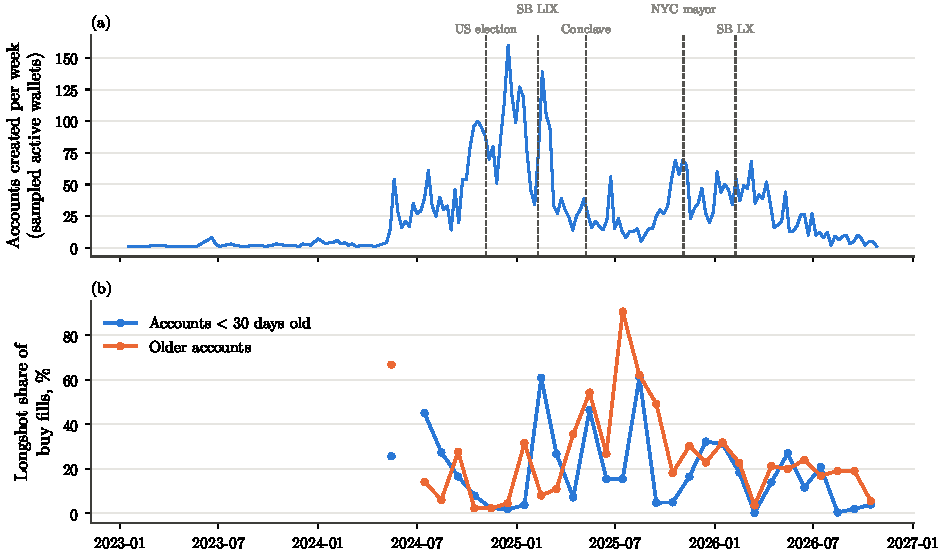
\includegraphics[width=\textwidth]{figures/fig_wallets_inflow.pdf}
\caption{Retail inflow and longshot buying. (a) Weekly account creations of the address-selected subset of sampled wallets, with five salient events marked. (b) Longshot share of design-weighted buy fills by accounts under 30 days old and by older accounts, by month (months with at least 30 fills), buy fills before the information time.}\label{fig:wallets-inflow}
\end{figure}

\subsubsection{The bias across venues}\label{sec:res-wallets-venues}

% source: data/research/flb_wallets/summary.json:xvenue, xvenue_gap.csv, xvenue_calib.csv
On 523 matched team-sides in 441 games, Kalshi and Polymarket agree almost exactly
before the start (\cref{tab:wallets-xvenue}, \cref{fig:wallets-xvenue}). One hour before the start the prices
correlate at 0.9993, and the mean absolute gap between the Polymarket price and the Kalshi midpoint is
0.40\cents. A day before it is 0.59\cents.

Game-winner markets rarely price a side at 10\cents{} or less an hour before the start: only 6
team-sides do, so the comparison cannot say whether one venue prices longshots higher. Between 11\cents{} and 80\cents{}
(495 team-sides), the mean gap in every bucket is within 0.05\cents{} of zero. Above 80\cents{}
(22 team-sides), Polymarket prices the favourite slightly below Kalshi's midpoint: by
0.59\cents{} at 90\cents{} or more
($t=-3.8$). Calibration slopes on the same team-sides are 0.71
for Kalshi and 0.71 for Polymarket ($t=-2.0$ and
$t=-2.0$ against one). The two are equal because the prices almost
coincide (\cref{tab:wallets-xvenue}). Gaps are short-lived:
\begin{itemize}
  \item the hour-to-hour autocorrelation of a pair's gap is 0.79, a half-life of about
    3.0 hours;
  \item the gap 24 hours out has a correlation of 0.09 with the gap an hour before the start.
\end{itemize}
Only 2.3\% of the one-hour gaps exceed the sum of the two venues' taker fees, and
0.2\% exceed fees plus Kalshi's half-spread. Within Polymarket,
\citet{saguillo2025} document arbitrage between related markets; across these two venues, price gaps on the
same games are almost always inside trading costs. We use no Polymarket US prices (\cref{sec:data-wallets}). By its
published schedule, a small Polymarket US account pays the highest taker fee of the three venues
(\cref{tab:wallets-fees}), so a gap involving that venue would have to be wider still to clear fees.

\begin{figure}[t]
\centering
% source: data/research/flb_wallets/xvenue_gap.csv
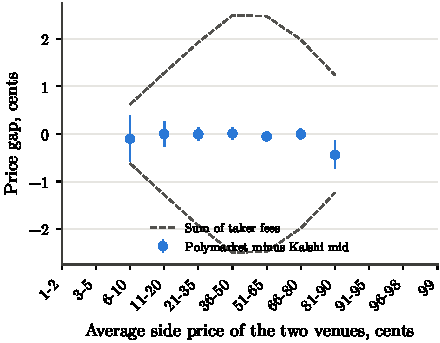
\includegraphics[width=0.55\textwidth]{figures/fig_wallets_xvenue.pdf}
\caption{Polymarket price minus Kalshi bid--ask midpoint for the same team, one hour before the scheduled start, by the two venues' average side price, with 95\% intervals clustered by game. Dashed: mean sum of the two venues' taker fees at those prices.}\label{fig:wallets-xvenue}
\end{figure}

\begin{table}[t]
\centering
\small
\begin{threeparttable}
\caption{Kalshi and Polymarket prices on the same games}\label{tab:wallets-xvenue}
% source: data/research/flb_wallets/summary.json:xvenue, xvenue_gap.csv, xvenue_calib.csv
\setlength{\tabcolsep}{4pt}
\begin{tabular}{rrrrrrrrrrrrr}
\toprule
Lead & Team & & Corr. & Mean $|g|$ & \multicolumn{2}{c}{$g$, $\bar q\le10\cents$} & \multicolumn{2}{c}{$g$, $\bar q\ge90\cents$} & \multicolumn{2}{c}{$|g|>$ fees (\%)} & \multicolumn{2}{c}{$\beta$} \\
\cmidrule(lr){6-7}\cmidrule(lr){8-9}\cmidrule(lr){10-11}\cmidrule(lr){12-13}
(h) & sides & Games & of prices & (\cents) & \cents & ($t$) & \cents & ($t$) & fees & +spread & Kalshi & PM \\
\midrule
1 & 523 & 441 & 0.9993 & 0.40 & $-$0.10 & ($-$0.5) & $-$0.59 & ($-$3.8) & 2.3 & 0.2 & 0.71 & 0.71 \\
3 & 523 & 441 & 0.9993 & 0.40 & $-$0.01 & ($-$0.0) & $-$0.04 & ($-$0.1) & 2.7 & 0.2 & 0.70 & 0.70 \\
6 & 523 & 441 & 0.9993 & 0.42 & $-$0.02 & ($-$0.1) & $-$0.12 & ($-$0.4) & 2.5 & 0.0 & 0.70 & 0.69 \\
12 & 523 & 441 & 0.9967 & 0.54 & $+$0.31 & (0.9) & $+$0.19 & (0.6) & 3.8 & 1.1 & 0.69 & 0.69 \\
24 & 514 & 432 & 0.9976 & 0.59 & $-$0.19 & ($-$0.4) & $+$0.23 & (0.6) & 4.9 & 0.6 & 0.69 & 0.69 \\
\bottomrule
\end{tabular}
\begin{tablenotes}\footnotesize
\item Kalshi NBA, NHL, NFL, college-football and WNBA game-winner markets (August--October 2026) matched to the
  same team's Polymarket outcome, observed on the same hourly timestamp $L$ hours before the scheduled
  start. $g=p^{\mathrm{PM}}-p^{\mathrm{K}}$ with $p^{\mathrm{K}}$ the Kalshi bid--ask midpoint; $\bar q$ is the two venues'
  average price of that side. Fees: Kalshi taker $0.07\,p(1-p)$ plus each Polymarket market's taker rate;
  ``+spread'' adds Kalshi's half-spread. $\beta$: calibration slope \eqref{eq:logit} on the same team-sides.
  $t$-statistics clustered by game.
\end{tablenotes}
\end{threeparttable}
\end{table}

\paragraph{Summary.}
On identified Polymarket wallets, the pattern predicted by \cref{hyp:pref} appears in who trades longshots, not
in who profits:
\begin{itemize}
  \item longshots are a large share of the buying of small wallets and market makers, and almost none of the
    buying of whales and mid-size wallets;
  \item small, occasional wallets are significant net buyers of longshots, and their buying is absorbed by
    all other classes, none of which is individually a significant net seller;
  \item new accounts put a smaller share of their buying into longshots than established ones, but lose
    almost all of what they put in;
  \item longshot buys lose about half their cost on average and favourite buys earn a few per cent;
  \item wallet profits are extremely concentrated, but they do not persist out of sample;
  \item Kalshi and Polymarket price the same games almost identically.
\end{itemize}
